% ++++++++++++++++++++++++++++++++++++++++
% Don't modify this section unless you know what you're doing!
\documentclass[a4paper,12pt]{article}
\usepackage{tabularx} % extra features for tabular environment
\usepackage{amsmath}  % improve math presentation
\usepackage{graphicx} % takes care of graphic including machinery
\usepackage[margin=0.75in]{geometry} % decreases margins
\usepackage{subcaption}
\usepackage{verbatim}
\usepackage{float}
\usepackage{hyperref}
\usepackage{titling}
\hypersetup{
	colorlinks=true,       % false: boxed links; true: colored links
	linkcolor=black,        % color of internal links
	citecolor=blue,        % color of links to bibliography
	filecolor=magenta,     % color of file links
	urlcolor=blue         
}
%++++++++++++++++++++++++++++++++++++++++
\setlength{\parindent}{0pt}
\setlength\parskip{0.5em plus 0.1em minus 0.2em}
\setlength{\droptitle}{-5em}   % This is your set screw

\begin{document}
\title{Charge to Mass Ratio for Electron \\
\large PHY224 Fall 2021}
\author{Fredrik Dahl Bråten, Pankaj Patil}
\date{\today}
\maketitle
\begin{center}
	\section*{Abstract}
\end{center}

In this variation of J. J. Thomson experiment, we aim to estimate the charge to mass ratio of the electron.
As predicted by the theory, we observe the deflection of moving charges in a magnetic field. The electrons are
deflected in such a way that they forms a circular trajectory, for which the radius can be measured. This
radius can then be used to measure the charge to mass ratio for the electron, with the help of theoretical formulas
relating the magnetic field to the radius of the orbit. 

\section{Introduction}

\subsection*{A. Background Theory}

An Electron moving with a velocity $\vec{v}$ through a magnetic field $\vec{B}$, experiences a force $\vec{F} = e\vec{v}\times \vec{V}$.
In a constant magnetic field, with a velocity perpendicular to it, the electron moves in a circular orbit, such that $evB = m\frac{v^2}{r}$.

When the electrons are accelerated through the potential $V$ in the electron gun, we have $eV = \frac{1}{2}mv^2$, which when combined with the former 
equation gives $\frac{1}{r} = \sqrt{\frac{e}{2m}} \frac{B}{\sqrt{V}}$.

By measuring the potential, the magnetic field and the radius of the orbit, we can determine the charge to mass ratio of the electron with the above formula. 

\subsection*{B. Materials and Methods}

The main apparatus' for the experiment are the two Helmholtz coils, which produce the magnetic field that bend the electron beam, 
the vacuum tube, filled by a low density gas for minimal electron resistance, though which gives some rare collitions which emit
light for visual inspection of the electron trajectory, and lastly the electron gun for creating the beam of free electrons with velocity v.

We followed the instructions given in the lab manual \cite{lab-manual-ex8}, and also the instructions given to us by the TA.

\section{Results}

To compute the external magnetic field, we use $\frac{1}{r} = \sqrt{\frac{e}{2m}}\frac{1}{\sqrt{V}}(B_c + B_e) \implies B_c = (constant)\frac{1}{r} - B_e$. 
The constant factor is due to measurements done with constant voltage. The intercept of the fitted line gives $B_e = 0.00001 \pm 0.00005$ Tesla.

\begin{figure}[H]
  \centering
  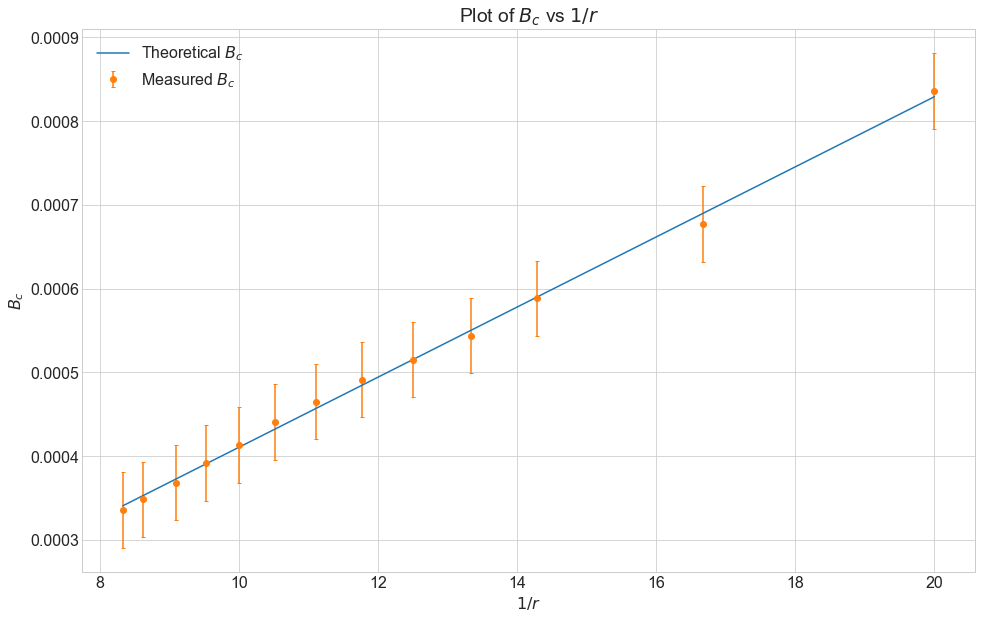
\includegraphics[width=0.8\linewidth]{../code/Pankaj/Coil B vs r_1.png} 
  \begin{center}
    Fitting Equation $f(x) = ax+b$ \\
    $B_e = -b$
  \end{center}  
    \caption{Computation of External Magnetic Field: $B_c$ vs $1/r$}
    \label{b_e}
\end{figure}

To compute the charge to mass ratio, we use $\frac{1}{r} = \sqrt{\frac{e}{m}}k\frac{I-I_0}{\sqrt{V}}$. For this case we use the data
obtained keeping current constant. The charge to mass ratio is give by $(\frac{slope}{k(I-I_0)})^2$. The charge to mass ratio
obtained in our case is $-(1.61 \pm 0.04) \times 10^{11}\ C/kg$.

\begin{figure}[H]
  \centering
  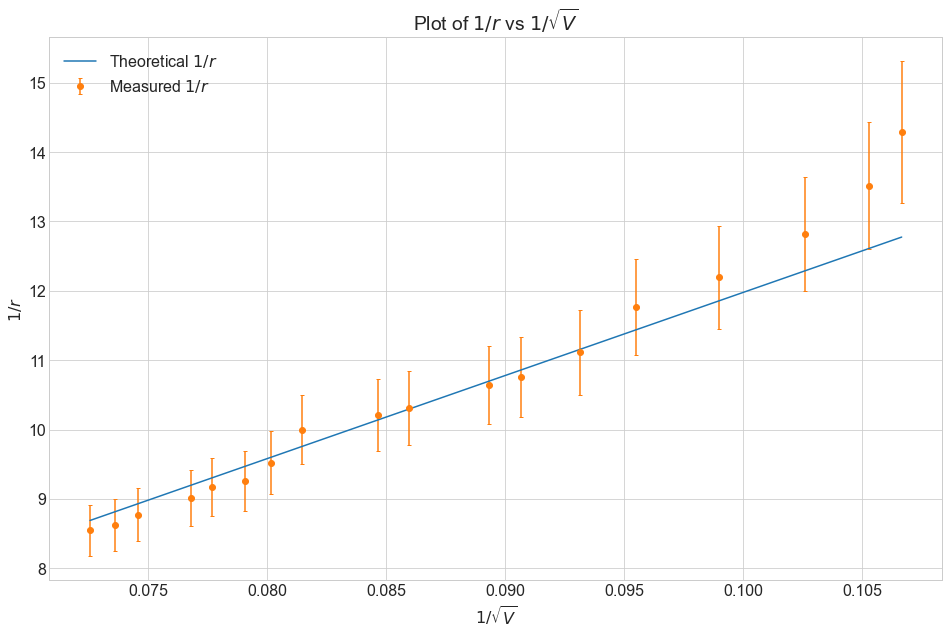
\includegraphics[width=0.8\linewidth]{../code/Pankaj/Charge To Mass Ratio.png}   
  \begin{center}
    Fitting Equation $f(x) = ax$ \\
    $a = 119.77$
  \end{center}   
  \caption{Computation of e/m: $1/r$ vs $1/\sqrt{V}$}
  \label{e_m}
\end{figure}

\section{Uncertainty}

For the calculation of $B_e$, the uncertainty is given by the fitting function. Hence $\Delta B_e = \Delta (y-intercept) = \pm 0.00005$ Tesla.

For the computation of the charge to mass ratio, we have $\frac{e}{m} = (\frac{slope}{k(I-I_0)})^2 \implies 
\Delta (\frac{e}{m}) = 2 (slope) \frac{\Delta (slope)}{(k(I-I_0))^2}$. The uncertainty is then $\Delta (\frac{e}{m}) = \pm 0.04 \times 10^{11}\ C/kg$.

\section{Discussion}


Weak potential limit: The beam of electrons becomes visible when the electrons have enough kinetic energy to excite the gas by collision. However, when one lowers the 
potential below a certain threshold, for which we found to be around 90 Volts, the electrons do no longer have enough energy to emit a visible 
photon during collisions with the gas. Thus the electron beam becomes invisible when the electron beam is accelerated by a voltage below about 90 volt.

Strong potential, weak magnetic field limit: In this case, the electrons are accelerated to a velocity so high that the magnetic field bending of the electron beam becomes negligible.
The electron beam then travels in a approximately straight line from the electron gun, perhaps weakly bent by the magnetic field, before the beam hits the wall on
the other end of the vacuum chamber.

In general, one will observe that as long as the potential is strong enough to make the beam trajectory visible, only the relative strength of the 
potential and the magnetic field matters. Without loss of generality, if we fix the potential and tune the strength of the magnetic field from low to high, 
we will see that the electron beam goes from forming a straight line through the chamber, to being bent and hitting the wall of the vacuum chamber lower 
and lower, until the beam closes in on itself and forms a circle with a certain radius. As we continue to increase the strength of the magnetic field, the 
electrons are accelerated more and more. Therefore the radius of the beam circle shrinks and shrinks. In the infinite strength limit, the radius 
converges to zero. 

In the case of low accelerating voltage and a strong magnetic field, we saw that the electron beam first is weakly bent downwards, close to the electron gun, 
and then gets more and more strongly bent as the beam approaches the centre of the vacuum chamber, and thus the maximum of the external magnetic field. This 
results in a non-circular electron beam trajectory. However this effect is small and not a significant source of error in our measurements, as we are still
able to estimate the radius of the trajectory reasonably well. What does however introduces a significant source of error in our estimation of the electrons 
charge to mass ratio, is that in this situation the circular beam trajectory is not centered at the centre of the chamber. This is because the electrons velocity 
is so low that the electrons never reach far enough into the chamber before being bent into traveling in the other direction. Therefore the centre of the 
circle is significantly far away from the centre of the chamber. Our measurements in this situation therefore underestimate the charge to mass ratio of the electron, 
as we have assumed the magnetic field to be constant within the chamber and equal to the magnetic field strength at the centre of the chamber. However, in this situation, 
the magnetic field strength at the centre of the trajectory is weaker than at the centre of the chamber by an amount calculable by the formulas in the manual. 
This implies the solution to our problem: We can reduce this error in our charge to mass ratio estimate by estimating the actual magnetic field strength at 
the centre of the trajectory of the electron beam, and use this magnetic field strength in our calculations of the charge to mass ratio.

When the light emitted by the electron beam hitting the gas reaches the curved walls of the vacuum chamber, the light is bent as it changes medium from low density gas, to glass
and then to air outside the chamber. Also due to the curved walls of the chamber, the light is bent according to Snells law. Therefore it is difficult to measure the actual radius 
of the electron beam. To avoid this problem of parallax, we let the used a self illuminated scale with a plastic reflector. 
The light from the self illuminated scale hits the mirror and is reflected such that an image of the scale appears within the vacuum chamber by the electron beam. This is because the 
light from the scale is reflected by first the mirror, then travels to the glass wall of the vacuum chamber and from there is reflected to our eyes. Thus the light from the scale is 
bent in the same manner as the light from the beam, so by comparing the beam within the vacuum chamber to the scale hologram also appearing within the chamber, one can accurately 
measure the radius of the electron beam.

When bringing ferromagnetic materials close to the vacuum chamber with the circular electron beam, such as our computers or phones with metal casings, we see that we somewhat
distort the magnetic field within the vacuum chamber. We know this because we can observe that the circular electron beam is weakly distorted into a different shape, for which depend
on the placement of the ferromagnetic material in relation to the chamber. Depending on the size and amount of ferromagnetic material we brought close to the vacuum chamber, 
the magnetic field and thus our measurements ranged from being negligibly affected, to being significantly affected. 


\pagebreak

\appendix

\section{Appendix}

\subsection{Experimental Data}

\subsubsection*{A Constant Current}

\noindent\rule{\textwidth}{1pt}
\verbatiminput{../data/Changing_voltage.csv}
\noindent\rule{\textwidth}{1pt}

\subsubsection*{B Constant Voltage}

\noindent\rule{\textwidth}{1pt}
\verbatiminput{../data/Changing_current.csv}
\noindent\rule{\textwidth}{1pt}

\pagebreak

\subsection{Python Code}

The Python code for this exercise is divided into two files. statslab.py file contains utility methods
which we will be frequently using in this course. lab\_8.py file contains the code which analyzes
the data.

\subsubsection{statslab.py}
\noindent\rule{\textwidth}{1pt}
\verbatiminput{../code/Pankaj/statslab.py}
\noindent\rule{\textwidth}{1pt}

\pagebreak

\subsubsection{lab\_8.py}
\noindent\rule{\textwidth}{1pt}
\verbatiminput{../code/Pankaj/lab_8.py}
\noindent\rule{\textwidth}{1pt}


\pagebreak

\begin{thebibliography}{99}

\bibitem{lab-manual-ex8} Charge to mass ratio for electron (e/m) - charge\_to\_mass.pdf (\url{https://q.utoronto.ca/courses/235154/files/15436313/download?wrap=1}).

\end{thebibliography}
  
  
\end{document}
